%
% Copyright (c) 2017 Intel Corporation
%
% Permission is hereby granted, free of charge, to any person obtaining a copy
% of this software and associated documentation files (the "Software"), to
% deal in the Software without restriction, including without limitation the
% rights to use, copy, modify, merge, publish, distribute, sublicense, and/or
% sell copies of the Software, and to permit persons to whom the Software is
% furnished to do so, subject to the following conditions:
%
% The above copyright notice and this permission notice shall be included in
% all copies or substantial portions of the Software.
%
% THE SOFTWARE IS PROVIDED "AS IS", WITHOUT WARRANTY OF ANY KIND, EXPRESS OR
% IMPLIED, INCLUDING BUT NOT LIMITED TO THE WARRANTIES OF MERCHANTABILITY,
% FITNESS FOR A PARTICULAR PURPOSE AND NONINFRINGEMENT. IN NO EVENT SHALL THE
% AUTHORS OR COPYRIGHT HOLDERS BE LIABLE FOR ANY CLAIM, DAMAGES OR OTHER
% LIABILITY, WHETHER IN AN ACTION OF CONTRACT, TORT OR OTHERWISE, ARISING
% FROM, OUT OF OR IN CONNECTION WITH THE SOFTWARE OR THE USE OR OTHER DEALINGS
% IN THE SOFTWARE.
%

\newcommand{\repoTopPath}{../../..}
\newcommand{\commonPreamblePath}{\repoTopPath/common/latex/common_preamble.tex}
\input \commonPreamblePath

%----BEGIN TYPESETTING----------------------------------------------------------
\begin{document}
\sffamily

% create our own title area rather than \begin{titlepage} or \maketitle
\begin{center}
\let\savethefootnote\thefootnote
\let\thefootnote\relax\footnote{Intel, and Quartus are trademarks of Intel Corporation or its subsidiaries in the U.S. and/or other countries.}
\addtocounter{footnote}{-1}
\let\thefootnote\savethefootnote
\hspace{-1em}
\let\savethefootnote\thefootnote
\let\thefootnote\relax\footnote{Other names and brands may be claimed as the property of others.}
\addtocounter{footnote}{-1}
\let\thefootnote\savethefootnote
\hspace{-1em}
\LARGE{My First HPS System}\\[1em]
\end{center}

\begin{flushleft}
\normalsize{PDF created: \today}\\
\normalsize{Validated using tools release: \TheToolsReleaseVersion}
\end{flushleft}

% make an entry in the PDF bookmarks for the TOC
\pdfbookmark[0]{Contents}{sumario_label}
% insert the default TOC format
\tableofcontents

%----NEW SECTION DEFINITION-----------------------------------------------------
\section*{Overview}
% must manually add TOC reference for unnumbered section
\addcontentsline{toc}{section}{Overview}
%----NEW SECTION DEFINITION-----------------------------------------------------

\begin{flushleft}
\noindent
This tutorial demonstrates how to instantiate and configure a Hard Processor System (HPS) component into a Qsys system.  Unlike other components in the prior \textquote{My First Qsys System} tutorial, the HPS component does not define any soft logic to be configured in the FPGA, rather, it allows the designer to configure the interfaces between the existing processor hardware on the SoC FPGA chip.  Configuring an entire processor system is a necessarily detailed process, but the level of customization available is precisely the advantage an SoC FPGA provides.  This tutorial shows as closely as possible how to set up the HPS in a similar manner to the design that shipped with the Terasic DE10-Nano board, and integrate it with the existing Qsys system from the preceding \textquote{My First Qsys System} tutorial.  This will allow us to integrate this example onto the existing SD card image that ships with the Terasic DE10-Nano board.

\end{flushleft}

%----NEW SECTION DEFINITION-----------------------------------------------------
\section*{Prerequisites}
% must manually add TOC reference for unnumbered section
\addcontentsline{toc}{section}{Prerequisites}
%----NEW SECTION DEFINITION-----------------------------------------------------

\begin{flushleft}
\noindent
The following are required:

\begin{itemize}

\item Windows\textsuperscript{*} or Linux\textsuperscript{*} development host PC

\item Installed Intel\textsuperscript{\textregistered} Quartus\textsuperscript{\textregistered} Prime Software Suite.  Either the Lite or Standard Edition, but not the Pro Edition.

\item Completed Intel Quartus software project from \textquote{My First Qsys System}

\begin{itemize}

\item Either follow the tutorial steps presented \href{\TheReleasesURL/writeup_MyFirstQsysSystem.pdf}{\underline{here}}.

%\item Or, you can extract this PDF attachment to your local file system: \textattachfile[
%	color=0.0 0.678 0.937,
%	mimetype=application/zip,
%	description={ZIP Archvie File: blink.zip}
%]{../blink_archive/blink.zip}{\textbf{blink.zip}}. Right click on the PDF attachment link and your PDF reader should present a pop-up menu with an option to save the attachment to your local file system.
\item Or, you can download an archive of the required contents from that tutorial to your local file system \href{\TheReleasesURL/blink_for_MyFirstHPSSystem.zip}{\underline{here}}.

\end{itemize}

\end{itemize}

\end{flushleft}

\newpage

%----NEW SECTION DEFINITION-----------------------------------------------------
\section*{Instantiating the Hard Processor System}
% must manually add TOC reference for unnumbered section
\addcontentsline{toc}{section}{Instantiating the Hard Processor System}
%----NEW SECTION DEFINITION-----------------------------------------------------

\begin{flushleft}
\noindent

This section will describe the steps required to instantiate an HPS core into the Qsys system that was created in the \textquote{My First Qsys System} tutorial.  It assumes that you have the completed \textbf{blink} project from that tutorial open.

\begin{enumerate}[
	label=\textbf{Step \arabic*.},
	leftmargin=*,
	widest={00},
	align=left]

\item With the \textbf{blink} project from the previous tutorial open in the Intel Quartus software tool, start by launching Qsys by clicking the Qsys button on the Intel Quartus software toolbar, or select Qsys from the \textbf{Tools} menu.  When the Qsys \textbf{Open} dialog appears select the \textbf{soc\_system.qsys} system and click the \textbf{Open} button.

\begin{figure}[H]
\centering
% screen shots report a density of 37.8 PixelsPerCentimeter when actual resolution
% is more like 56 PixelsPerCentimeter, so the scaling factor for 1:1 is 0.675
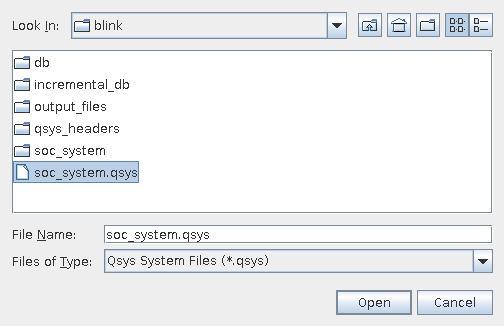
\includegraphics[scale=0.675]{01-open-qsys}
\caption{Qsys Open Dialog}
\label{fig:01-open-qsys}
\end{figure}

\item In the \textbf{IP Catalog}, search for \textbf{hard processor} and double click on \textbf{Arria V/Cyclone V Hard Processor System} to bring up the HPS component configuration wizard.

\begin{figure}[H]
\centering
% screen shots report a density of 37.8 PixelsPerCentimeter when actual resolution
% is more like 56 PixelsPerCentimeter, so the scaling factor for 1:1 is 0.675
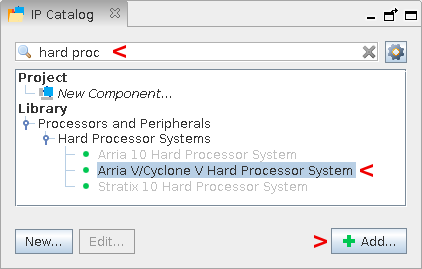
\includegraphics[scale=0.675]{02-hps-search}
\caption{Hard Processor Search}
\label{fig:02-hps-search}
\end{figure}

\newpage

\item On the \textbf{FPGA Interfaces} tab in the \textbf{General} section, deselect the \textbf{Enable MPU standby and event signals} parameter.

It should look like this after you do.

\begin{figure}[H]
\centering
% screen shots report a density of 37.8 PixelsPerCentimeter when actual resolution
% is more like 56 PixelsPerCentimeter, so the scaling factor for 1:1 is 0.675
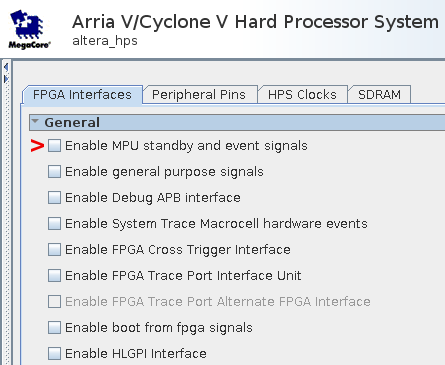
\includegraphics[scale=0.675]{03-fpga-int-general}
\caption{FPGA Interfaces - General}
\label{fig:03-fpga-int-general}
\end{figure}

\item In the \textbf{AXI Bridges} section, select \textbf{unused} for the \textbf{FPGA-to-HPS interface width} parameter.

It should look like this after you do.

\begin{figure}[H]
\centering
% screen shots report a density of 37.8 PixelsPerCentimeter when actual resolution
% is more like 56 PixelsPerCentimeter, so the scaling factor for 1:1 is 0.675
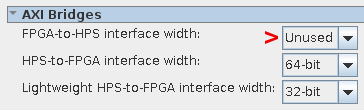
\includegraphics[scale=0.675]{04-fpga-int-axi-bridges}
\caption{AXI Bridges}
\label{fig:04-fpga-int-axi-bridges}
\end{figure}

\item In the \textbf{FPGA-to-HPS SDRAM Interface} section, select the \textbf{f2h\_sdram0} interface and click the \textbf{-} button to remove it from the list.

It should look like this after you do.

\begin{figure}[H]
\centering
% screen shots report a density of 37.8 PixelsPerCentimeter when actual resolution
% is more like 56 PixelsPerCentimeter, so the scaling factor for 1:1 is 0.675
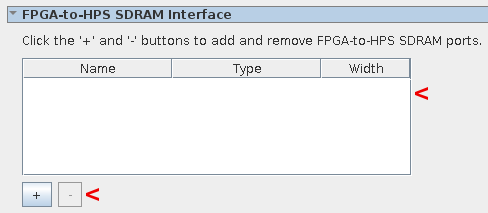
\includegraphics[scale=0.675]{05-fpga-int-f2s-bridge}
\caption{FPGA-to-HPS SDRAM Interface}
\label{fig:05-fpga-int-f2s-bridge}
\end{figure}

\newpage

\item In the \textbf{Resets} section, do not change any of the default settings.

\begin{figure}[H]
\centering
% screen shots report a density of 37.8 PixelsPerCentimeter when actual resolution
% is more like 56 PixelsPerCentimeter, so the scaling factor for 1:1 is 0.675
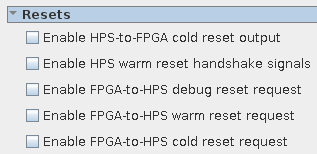
\includegraphics[scale=0.675]{06-fpga-int-resets}
\caption{Resets}
\label{fig:06-fpga-int-resets}
\end{figure}

\item In the \textbf{DMA Peripheral Request} section, do not change any of the default settings.

\begin{figure}[H]
\centering
% screen shots report a density of 37.8 PixelsPerCentimeter when actual resolution
% is more like 56 PixelsPerCentimeter, so the scaling factor for 1:1 is 0.675
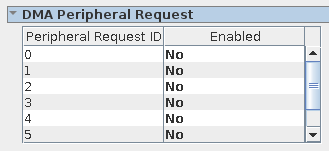
\includegraphics[scale=0.675]{07-fpga-int-dma}
\caption{DMA Peripheral Request}
\label{fig:07-fpga-int-dma}
\end{figure}

\item In the \textbf{Interrupts} section, do not change any of the default settings.

\begin{figure}[H]
\centering
% screen shots report a density of 37.8 PixelsPerCentimeter when actual resolution
% is more like 56 PixelsPerCentimeter, so the scaling factor for 1:1 is 0.675
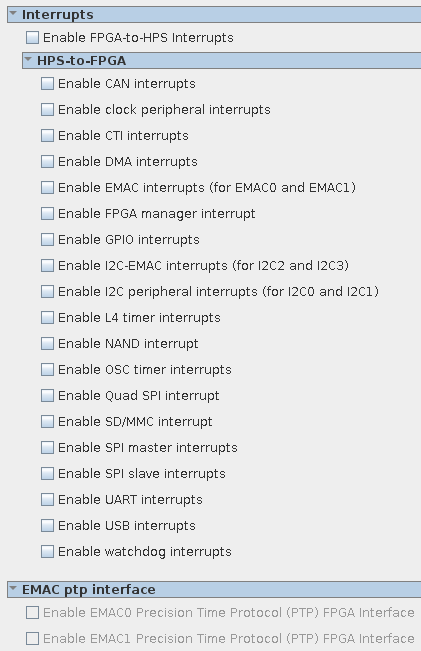
\includegraphics[scale=0.675]{08-fpga-int-interrupts}
\caption{Interrupts}
\label{fig:08-fpga-int-interrupts}
\end{figure}

\newpage

\item On the \textbf{Peripheral Pins} tab in the \textbf{Ethernet Media Access Controller} section, make the following changes:

\begin{enumerate}[
	label=\textbf{Step \arabic{enumi}\alph*.},
	leftmargin=*,
	align=left]

\item Select \textbf{HPS I/O Set 0} for the \textbf{EMAC1 pin} parameter.

\item Select \textbf{RGMII} for the \textbf{EMAC1 mode} parameter.

\end{enumerate}

It should look like this after you do.

\begin{figure}[H]
\centering
% screen shots report a density of 37.8 PixelsPerCentimeter when actual resolution
% is more like 56 PixelsPerCentimeter, so the scaling factor for 1:1 is 0.675
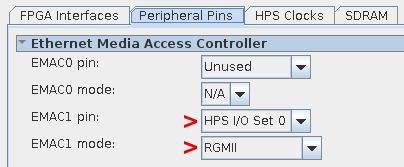
\includegraphics[scale=0.675]{09-periph-emac}
\caption{Ethernet Media Access Controller}
\label{fig:09-periph-emac}
\end{figure}

\item In the \textbf{NAND Flash Controller} section, do not change any of the default settings.

\begin{figure}[H]
\centering
% screen shots report a density of 37.8 PixelsPerCentimeter when actual resolution
% is more like 56 PixelsPerCentimeter, so the scaling factor for 1:1 is 0.675
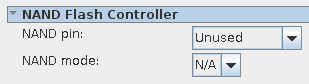
\includegraphics[scale=0.675]{10-periph-nand}
\caption{NAND Flash Controller}
\label{fig:10-periph-nand}
\end{figure}

\item In the \textbf{Quad SPI Flash Controller} section, do not change any of the default settings.

\begin{figure}[H]
\centering
% screen shots report a density of 37.8 PixelsPerCentimeter when actual resolution
% is more like 56 PixelsPerCentimeter, so the scaling factor for 1:1 is 0.675
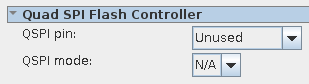
\includegraphics[scale=0.675]{11-periph-qspi}
\caption{Quad SPI Flash Controller}
\label{fig:11-periph-qspi}
\end{figure}

\item In the \textbf{SD/MMC Controller} section, make the following changes:

\begin{enumerate}[
	label=\textbf{Step \arabic{enumi}\alph*.},
	leftmargin=*,
	align=left]

\item Select \textbf{HPS I/O Set 0} for the \textbf{SDIO pin} parameter.

\item Select \textbf{4-bit Data} for the \textbf{SDIO mode} parameter.

\end{enumerate}

It should look like this after you do.

\begin{figure}[H]
\centering
% screen shots report a density of 37.8 PixelsPerCentimeter when actual resolution
% is more like 56 PixelsPerCentimeter, so the scaling factor for 1:1 is 0.675
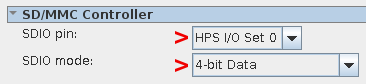
\includegraphics[scale=0.675]{12-periph-sdmmc}
\caption{SD/MMC Controller}
\label{fig:12-periph-sdmmc}
\end{figure}

\newpage

\item In the \textbf{USB Controllers} section, make the following changes:

\begin{enumerate}[
	label=\textbf{Step \arabic{enumi}\alph*.},
	leftmargin=*,
	align=left]

\item Select \textbf{HPS I/O Set 0} for the \textbf{USB1 pin} parameter.

\item Select \textbf{SDR with PHY clock output mode} for the \textbf{USB1 PHY interface mode} parameter.

\end{enumerate}

It should look like this after you do.

\begin{figure}[H]
\centering
% screen shots report a density of 37.8 PixelsPerCentimeter when actual resolution
% is more like 56 PixelsPerCentimeter, so the scaling factor for 1:1 is 0.675
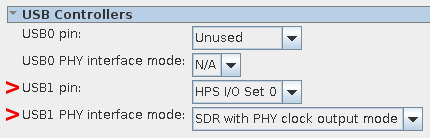
\includegraphics[scale=0.675]{13-periph-usb}
\caption{USB Controllers}
\label{fig:13-periph-usb}
\end{figure}

\item In the \textbf{SPI Controllers} section, make the following changes:

\begin{enumerate}[
	label=\textbf{Step \arabic{enumi}\alph*.},
	leftmargin=*,
	align=left]

\item Select \textbf{HPS I/O Set 0} for the \textbf{SPIM1 pin} parameter.

\item Select \textbf{Single Slave Select} for the \textbf{SPIM1 mode} parameter.

\end{enumerate}

It should look like this after you do.

\begin{figure}[H]
\centering
% screen shots report a density of 37.8 PixelsPerCentimeter when actual resolution
% is more like 56 PixelsPerCentimeter, so the scaling factor for 1:1 is 0.675
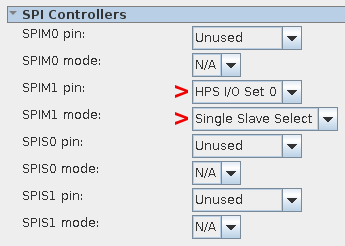
\includegraphics[scale=0.675]{14-periph-spi}
\caption{SPI Controllers}
\label{fig:14-periph-spi}
\end{figure}

\item In the \textbf{UART Controllers} section, make the following changes:

\begin{enumerate}[
	label=\textbf{Step \arabic{enumi}\alph*.},
	leftmargin=*,
	align=left]

\item Select \textbf{HPS I/O Set 0} for the \textbf{UART0 pin} parameter.

\item Select \textbf{No Flow Control} for the \textbf{UART0 mode} parameter.

\end{enumerate}

It should look like this after you do.

\begin{figure}[H]
\centering
% screen shots report a density of 37.8 PixelsPerCentimeter when actual resolution
% is more like 56 PixelsPerCentimeter, so the scaling factor for 1:1 is 0.675
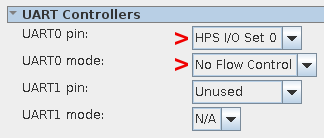
\includegraphics[scale=0.675]{15-periph-uart}
\caption{UART Controllers}
\label{fig:15-periph-uart}
\end{figure}

\newpage

\item In the \textbf{I2C Controllers} section, make the following changes:

\begin{enumerate}[
	label=\textbf{Step \arabic{enumi}\alph*.},
	leftmargin=*,
	align=left]

\item Select \textbf{HPS I/O Set 0} for the \textbf{I2C0 pin}  parameter.

\item Select \textbf{HPS I/O Set 0} for the \textbf{I2C1 pin}  parameter.

\item Select \textbf{I2C} for the \textbf{I2C0 mode}  parameter.

\item Select \textbf{I2C} for the \textbf{I2C1 mode} parameter.

\end{enumerate}

It should look like this after you do.

\begin{figure}[H]
\centering
% screen shots report a density of 37.8 PixelsPerCentimeter when actual resolution
% is more like 56 PixelsPerCentimeter, so the scaling factor for 1:1 is 0.675
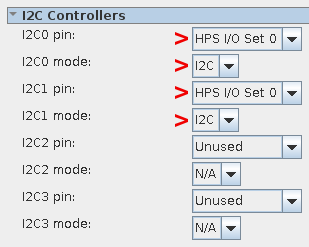
\includegraphics[scale=0.675]{16-periph-i2c}
\caption{I2C Controllers}
\label{fig:16-periph-i2c}
\end{figure}

\item In the \textbf{CAN Controllers} section, do not change any of the default settings.

\begin{figure}[H]
\centering
% screen shots report a density of 37.8 PixelsPerCentimeter when actual resolution
% is more like 56 PixelsPerCentimeter, so the scaling factor for 1:1 is 0.675
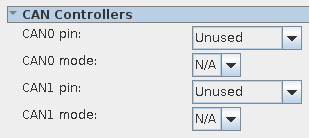
\includegraphics[scale=0.675]{17-periph-can}
\caption{CAN Controllers}
\label{fig:17-periph-can}
\end{figure}

\item In the \textbf{Trace Port Interface Unit} section, do not change any of the default settings.

\begin{figure}[H]
\centering
% screen shots report a density of 37.8 PixelsPerCentimeter when actual resolution
% is more like 56 PixelsPerCentimeter, so the scaling factor for 1:1 is 0.675
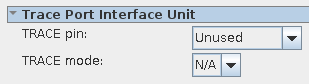
\includegraphics[scale=0.675]{18-periph-trace}
\caption{Trace Port Interface Unit}
\label{fig:18-periph-trace}
\end{figure}

\newpage

\item In the \textbf{Peripherals Mux Table} section, enable the following GPIO ports by clicking on the GPIOxx button in the second column from the right of the table.  Select the following GPIO:

\begin{itemize}

\item \textbf{GPIO09}

\item \textbf{GPIO35}

\item \textbf{GPIO40}

\item \textbf{GPIO53}

\item \textbf{GPIO54}

\item \textbf{GPIO61}

\end{itemize}

\begin{figure}[H]
\centering
% screen shots report a density of 37.8 PixelsPerCentimeter when actual resolution
% is more like 56 PixelsPerCentimeter, so the scaling factor for 1:1 is 0.675
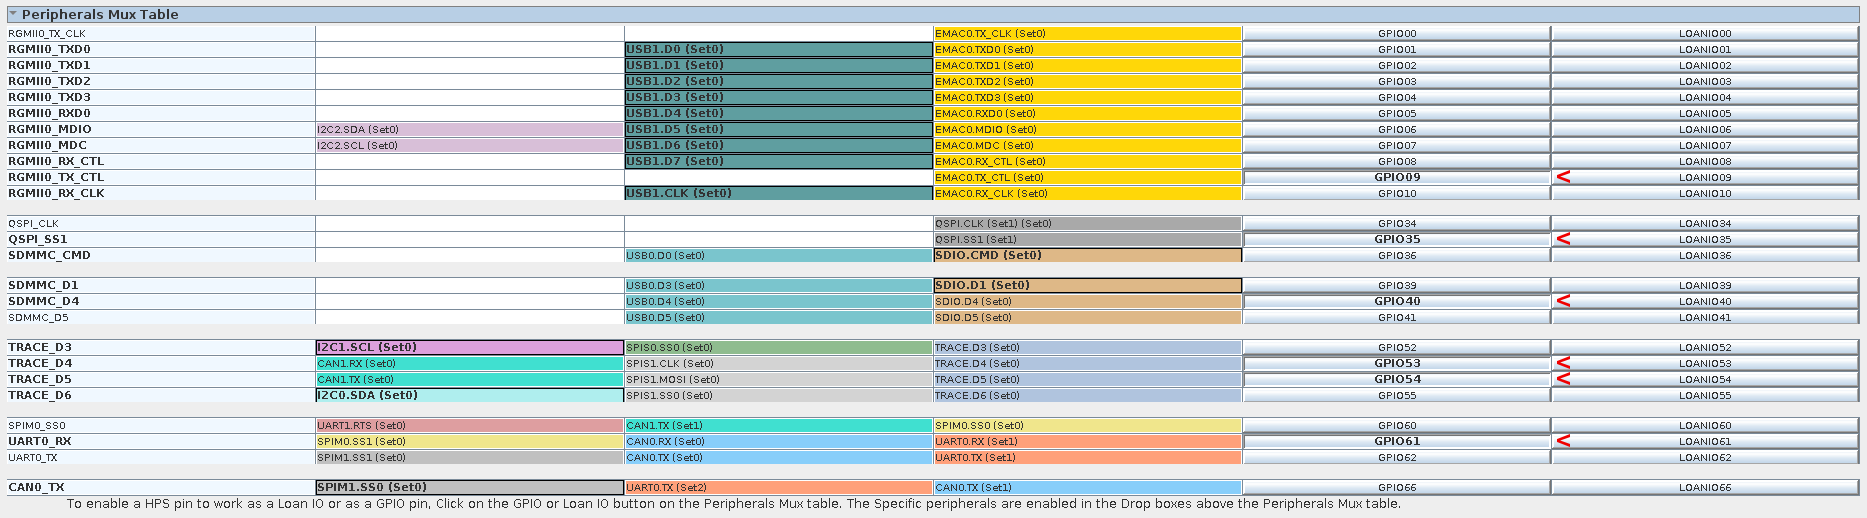
\includegraphics[scale=0.375]{19-periph-mux}
\caption{Peripherals Mux Table}
\label{fig:19-periph-mux}
\end{figure}

\item Moving on to the \textbf{HPS Clocks} tab, under the \textbf{Input Clocks} sub-tab, in the \textbf{External Clock Sources} section, do not change any of the default settings.

\begin{figure}[H]
\centering
% screen shots report a density of 37.8 PixelsPerCentimeter when actual resolution
% is more like 56 PixelsPerCentimeter, so the scaling factor for 1:1 is 0.675
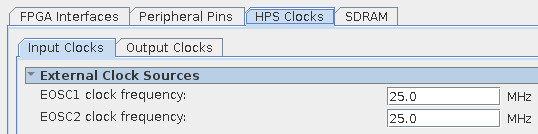
\includegraphics[scale=0.675]{20-hps-clks-in-external}
\caption{External Clock Sources}
\label{fig:20-hps-clks-in-external}
\end{figure}

\item In the \textbf{FPGA-to-HPS PLL Reference Clocks} section, do not change any of the default settings.

\begin{figure}[H]
\centering
% screen shots report a density of 37.8 PixelsPerCentimeter when actual resolution
% is more like 56 PixelsPerCentimeter, so the scaling factor for 1:1 is 0.675
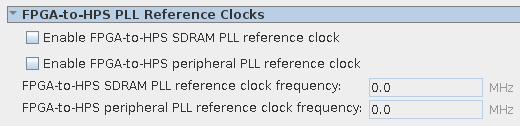
\includegraphics[scale=0.675]{21-hps-clks-in-fpga2hps}
\caption{FPGA-to-HPS PLL Reference Clocks}
\label{fig:21-hps-clks-in-fpga2hps}
\end{figure}

\newpage

\item In the \textbf{Peripheral FPGA Clocks} section, do not change any of the default settings.

\begin{figure}[H]
\centering
% screen shots report a density of 37.8 PixelsPerCentimeter when actual resolution
% is more like 56 PixelsPerCentimeter, so the scaling factor for 1:1 is 0.675
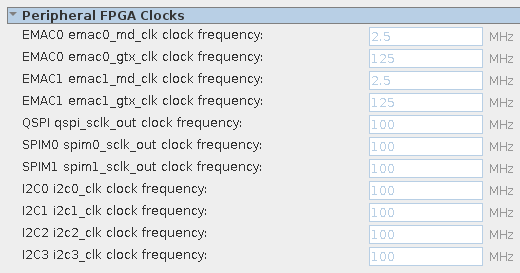
\includegraphics[scale=0.675]{22-hps-clks-in-peripheral-fpga}
\caption{Peripheral FPGA Clocks}
\label{fig:22-hps-clks-in-peripheral-fpga}
\end{figure}

\item Moving on to the \textbf{Output Clocks} sub-tab, in the \textbf{Clock Sources} section, do not change any of the default settings.

\begin{figure}[H]
\centering
% screen shots report a density of 37.8 PixelsPerCentimeter when actual resolution
% is more like 56 PixelsPerCentimeter, so the scaling factor for 1:1 is 0.675
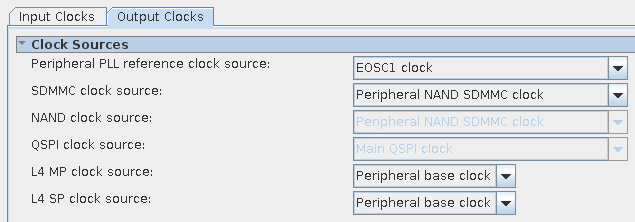
\includegraphics[scale=0.675]{23-hps-clks-out-clk-srcs}
\caption{Clock Sources}
\label{fig:23-hps-clks-out-clk-srcs}
\end{figure}

\item In the \textbf{Main PLL Output Clocks} section, do not change any of the default settings.

\begin{figure}[H]
\centering
% screen shots report a density of 37.8 PixelsPerCentimeter when actual resolution
% is more like 56 PixelsPerCentimeter, so the scaling factor for 1:1 is 0.675
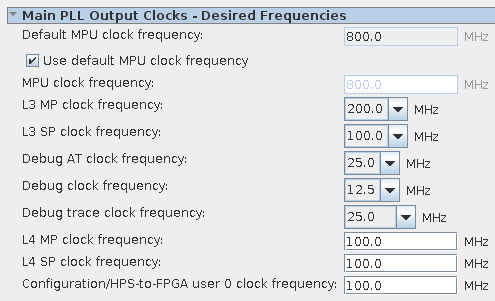
\includegraphics[scale=0.675]{24-hps-clks-out-main-pll}
\caption{Main PLL Output Clocks}
\label{fig:24-hps-clks-out-main-pll}
\end{figure}

\newpage

\item In the \textbf{Peripheral PLL Output Clocks} section, do not change any of the default settings.

\begin{figure}[H]
\centering
% screen shots report a density of 37.8 PixelsPerCentimeter when actual resolution
% is more like 56 PixelsPerCentimeter, so the scaling factor for 1:1 is 0.675
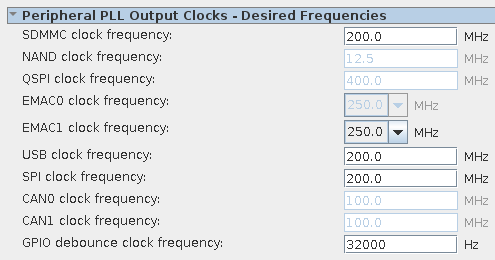
\includegraphics[scale=0.675]{25-hps-clks-out-periph-pll}
\caption{Peripheral PLL Output Clocks}
\label{fig:25-hps-clks-out-periph-pll}
\end{figure}

\item In the \textbf{HPS-to-FPGA User Clocks} section, do not change any of the default settings.

\begin{figure}[H]
\centering
% screen shots report a density of 37.8 PixelsPerCentimeter when actual resolution
% is more like 56 PixelsPerCentimeter, so the scaling factor for 1:1 is 0.675
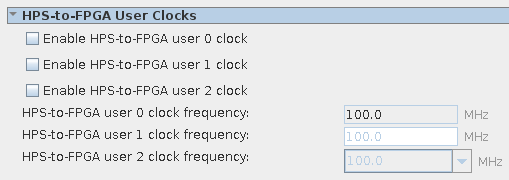
\includegraphics[scale=0.675]{26-hps-clks-out-h2f-user}
\caption{HPS-to-FPGA User Clocks}
\label{fig:26-hps-clks-out-h2f-user}
\end{figure}

\item Moving on to the \textbf{SDRAM} tab, under the \textbf{PHY Settings} sub-tab, in the \textbf{Clocks} section,  make the following changes:

\begin{enumerate}[
	label=\textbf{Step \arabic{enumi}\alph*.},
	leftmargin=*,
	align=left]

\item Change the \textbf{Memory clock frequency} parameter to \textbf{400.0}.

\item Change the \textbf{PLL reference clock frequency} parameter to \textbf{25.0}.

\end{enumerate}

It should look like this after you do.

\begin{figure}[H]
\centering
% screen shots report a density of 37.8 PixelsPerCentimeter when actual resolution
% is more like 56 PixelsPerCentimeter, so the scaling factor for 1:1 is 0.675
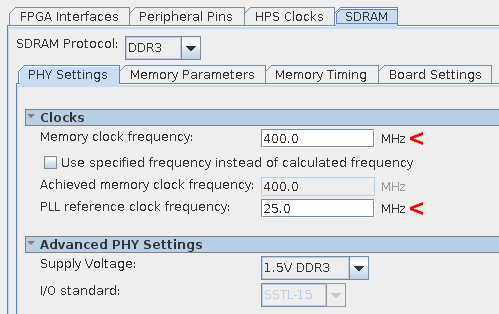
\includegraphics[scale=0.675]{27-sdram-phy}
\caption{PHY Settings}
\label{fig:27-sdram-phy}
\end{figure}

\newpage

\item Moving on to the \textbf{Memory Parameters} sub-tab, make the following changes:

\begin{enumerate}[
	label=\textbf{Step \arabic{enumi}\alph*.},
	leftmargin=*,
	align=left]

\item Change the \textbf{Memory vendor} parameter to \textbf{Other}.

\item Change the \textbf{Memory device speed grade} parameter to \textbf{800.0}.

\item Change the \textbf{Total interface width} parameter to \textbf{32}.

\item Change the \textbf{Row address width} parameter to \textbf{15}.

\item Change the \textbf{Column address width} parameter to \textbf{10}.

\end{enumerate}

It should look like this after you do.

\begin{figure}[H]
\centering
% screen shots report a density of 37.8 PixelsPerCentimeter when actual resolution
% is more like 56 PixelsPerCentimeter, so the scaling factor for 1:1 is 0.675
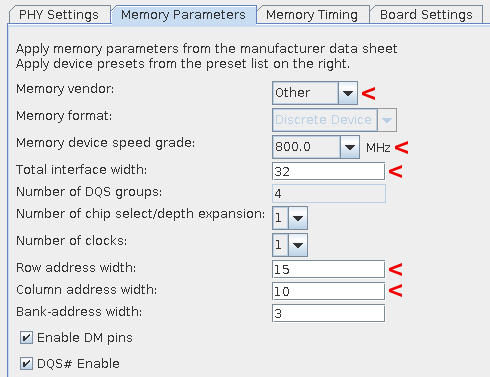
\includegraphics[scale=0.675]{28-sdram-param}
\caption{Memory Parameters}
\label{fig:28-sdram-param}
\end{figure}

\item In the \textbf{Memory Initialization Options} section:

\begin{enumerate}[
	label=\textbf{Step \arabic{enumi}\alph*.},
	leftmargin=*,
	align=left]

\item Change the \textbf{ODT Rtt nominal value} parameter to \textbf{RZQ/6}.

\item Change the \textbf{Memory write CAS latency setting} parameter to \textbf{7}.

\end{enumerate}

It should look like this after you do.

\begin{figure}[H]
\centering
% screen shots report a density of 37.8 PixelsPerCentimeter when actual resolution
% is more like 56 PixelsPerCentimeter, so the scaling factor for 1:1 is 0.675
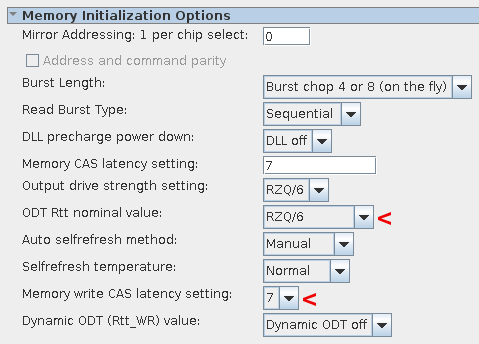
\includegraphics[scale=0.675]{29-sdram-param-init}
\caption{Memory Initialization Options}
\label{fig:29-sdram-param-init}
\end{figure}

\newpage

\item Moving on to the \textbf{Memory Timing} sub-tab, make the following changes:

\begin{enumerate}[
	label=\textbf{Step \arabic{enumi}\alph*.},
	leftmargin=*,
	align=left]

\item Change the \textbf{tINIT} parameter to \textbf{500}.

\item Change the \textbf{tMRD (tMRW)} parameter to \textbf{4}.

\item Change the \textbf{tRAS} parameter to \textbf{35.0}.

\item Change the \textbf{tRCD} parameter to \textbf{13.75}.

\item Change the \textbf{tRP} parameter to \textbf{13.75}.

\item Change the \textbf{tREFI (tREFIab)} parameter to \textbf{7.8}.

\item Change the \textbf{tRFC (tRFCab)} parameter to \textbf{300.0}.

\item Change the \textbf{tWTR} parameter to \textbf{4}.

\end{enumerate}

It should look like this after you do.

\begin{figure}[H]
\centering
% screen shots report a density of 37.8 PixelsPerCentimeter when actual resolution
% is more like 56 PixelsPerCentimeter, so the scaling factor for 1:1 is 0.675
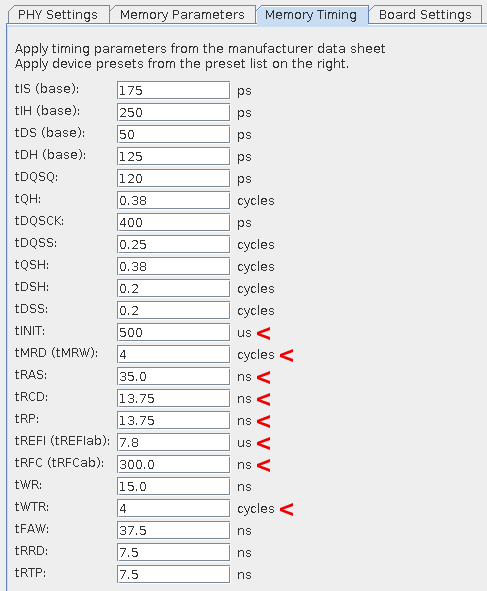
\includegraphics[scale=0.675]{30-sdram-timing}
\caption{Memory Timing}
\label{fig:30-sdram-timing}
\end{figure}

\newpage

\item Moving on to the \textbf{Board Settings} tab, in the \textbf{Setup and Hold Derating} section, do not change any of the default settings.

\begin{figure}[H]
\centering
% screen shots report a density of 37.8 PixelsPerCentimeter when actual resolution
% is more like 56 PixelsPerCentimeter, so the scaling factor for 1:1 is 0.675
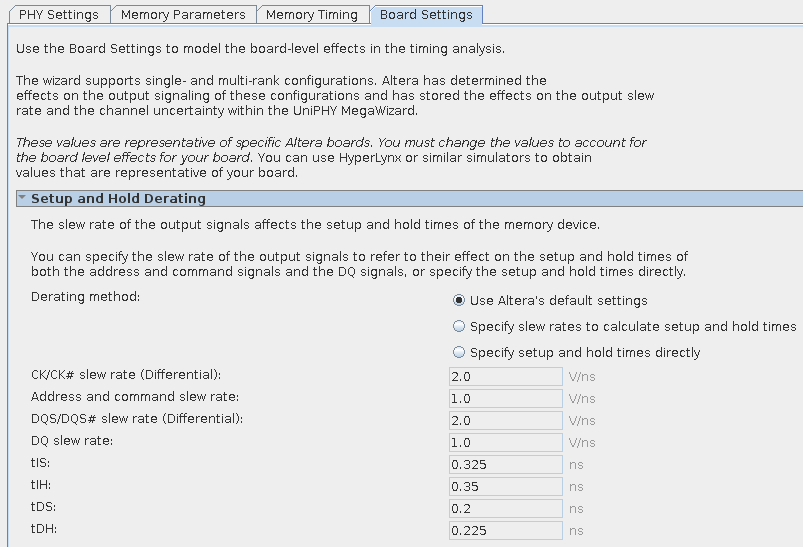
\includegraphics[scale=0.675]{31-sdram-board}
\caption{Setup and Hold Derating}
\label{fig:31-sdram-board}
\end{figure}

\item In the \textbf{Channel Signal Integrity} section, do not change any of the default settings.

\begin{figure}[H]
\centering
% screen shots report a density of 37.8 PixelsPerCentimeter when actual resolution
% is more like 56 PixelsPerCentimeter, so the scaling factor for 1:1 is 0.675
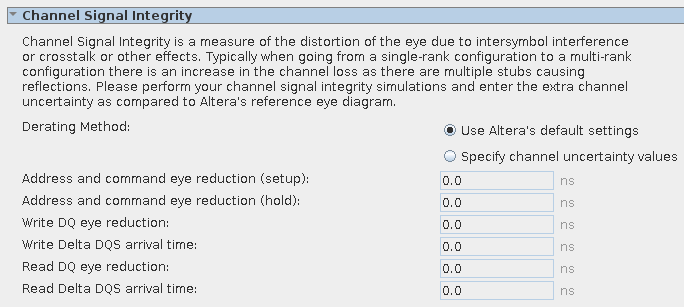
\includegraphics[scale=0.675]{32-sdram-board-sig-int}
\caption{Channel Signal Integrity}
\label{fig:32-sdram-board-sig-int}
\end{figure}

\newpage

\item In the \textbf{Board Skews} section, do not change any of the default settings.

\begin{figure}[H]
\centering
% screen shots report a density of 37.8 PixelsPerCentimeter when actual resolution
% is more like 56 PixelsPerCentimeter, so the scaling factor for 1:1 is 0.675
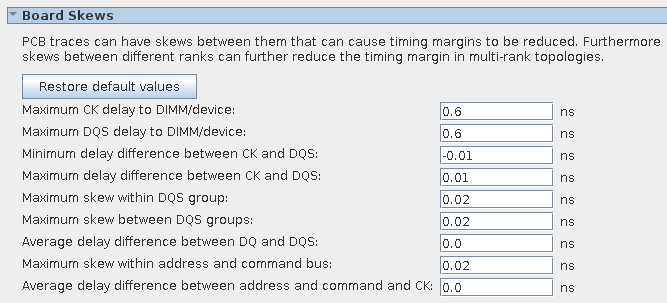
\includegraphics[scale=0.675]{33-sdram-board-skews}
\caption{Board Skews}
\label{fig:33-sdram-board-skews}
\end{figure}

\item The HPS configuration is now complete, you can click the \textbf{Finish} button in the bottom right corner of the dialog window.

\item The HPS instance appears in the system with the default name \textbf{hps\_0} which we will keep that way.  The \textbf{memory} conduit interface should already be exported with the name \textbf{memory} in the export column as well as the \textbf{hps\_io} conduit interface named \textbf{hps\_io} in the export column.  Rename the \textbf{hps\_io} conduit export name to \textbf{hps\_0\_hps\_io}

It should look like this after you do.

\begin{figure}[H]
\centering
% screen shots report a density of 37.8 PixelsPerCentimeter when actual resolution
% is more like 56 PixelsPerCentimeter, so the scaling factor for 1:1 is 0.675
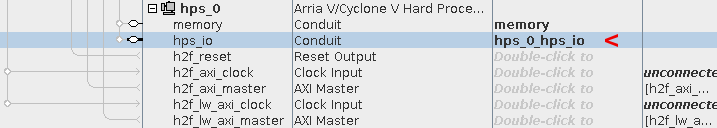
\includegraphics[scale=0.675]{34-hps-instance}
\caption{Board Skews}
\label{fig:34-hps-instance}
\end{figure}

\newpage

\item Complete the HPS connections into the rest of the system:

\begin{enumerate}[
	label=\textbf{Step \arabic{enumi}\alph*.},
	leftmargin=*,
	align=left]

\item Connect the \textbf{h2f\_axi\_clock} clock input to the \textbf{clk\_0} clock output.

\item Connect the \textbf{h2f\_lw\_axi\_clock} clock input to the \textbf{clk\_0} clock output.

\item Connect the \textbf{h2f\_reset} reset output to the reset input of all the other components.

\item Connect the \textbf{h2f\_axi\_master} AXI Master to the \textbf{ocram\_64k/s1} Avalon Slave.

\item Connect the \textbf{h2f\_axi\_master} AXI Master to the \textbf{default\_16b/s1} Avalon Slave.

\item Connect the \textbf{h2f\_lw\_axi\_master} AXI Master to the \textbf{default\_16b/s1} Avalon Slave.

\item Connect the \textbf{h2f\_lw\_axi\_master} AXI Master to the \textbf{led\_pio/s1} Avalon Slave.

\item Connect the \textbf{h2f\_lw\_axi\_master} AXI Master to the \textbf{button\_pio/s1} Avalon Slave.

\item Connect the \textbf{h2f\_lw\_axi\_master} AXI Master to the \textbf{switch\_pio/s1} Avalon Slave.

\item Connect the \textbf{h2f\_lw\_axi\_master} AXI Master to the \textbf{system\_id/control\_slave} Avalon Slave.

\end{enumerate}

It should look like this after you do.

\begin{figure}[H]
\centering
% screen shots report a density of 37.8 PixelsPerCentimeter when actual resolution
% is more like 56 PixelsPerCentimeter, so the scaling factor for 1:1 is 0.675
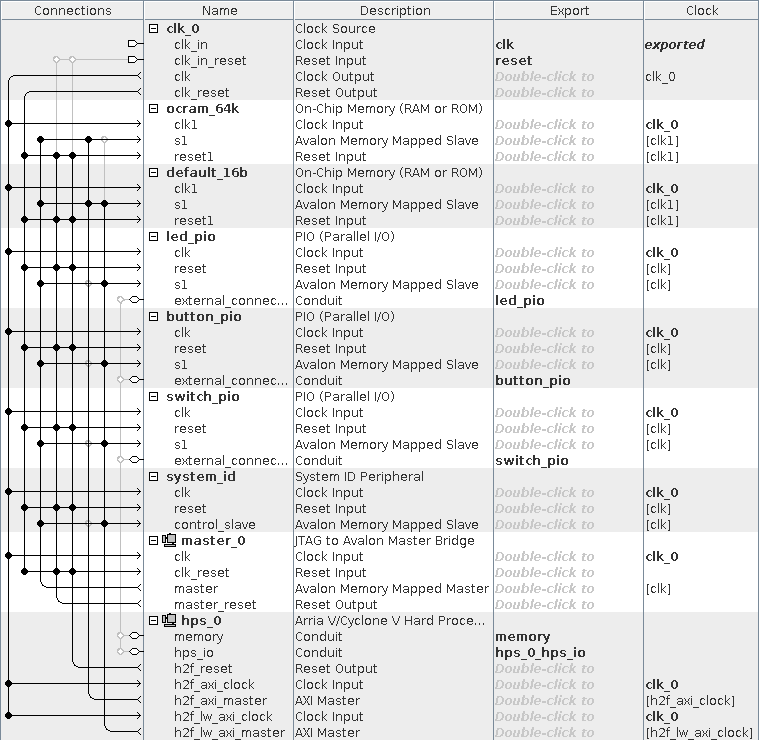
\includegraphics[scale=0.675]{35-hps-system}
\caption{Board Skews}
\label{fig:35-hps-system}
\end{figure}

\item Save the system, generate the HDL, and close Qsys.

\end{enumerate}

\end{flushleft}

%----NEW SECTION DEFINITION-----------------------------------------------------
\section*{Integrating the Qsys System into the Intel Quartus Software Project}
% must manually add TOC reference for unnumbered section
\addcontentsline{toc}{section}{Integrating the Qsys System into the Intel Quartus Software Project}
%----NEW SECTION DEFINITION-----------------------------------------------------

\begin{flushleft}
\noindent

This section will describe how to incorporate the newly generated Qsys output into the existing \textbf{blink} Intel Quartus software project.

\begin{enumerate}[
	label=\textbf{Step \arabic*.},
	leftmargin=*,
	widest={00},
	align=left]

\item Update the \textbf{blink.v} source file with the new code for the Qsys system instantiation like this:
\newline
\newline
%Extract PDF Attachment: \textattachfile[
%	color=0.0 0.678 0.937,
%	mimetype=text/plain,
%	description={Verilog Source File: blink.v}
%]{../../hdl_src/blink.v}{\textbf{blink.v}}
Download the blink.v file \href{\TheRawURL/MyFirstHPSSystem/hdl_src/blink.v}{\underline{here}}.
\newline
If you wish to view the blink.v file in the GitHub\textsuperscript{*} repo you can look \href{\TheBlobURL/MyFirstHPSSystem/hdl_src/blink.v}{\underline{here}}.

\inputminted[
	bgcolor=MyMintedBGColor,
	linenos,
	fontsize=\small
]{verilog}{../../hdl_src/blink.v}

\item Click the \textbf{Start Analysis \& Synthesis} button on the Intel Quartus software toolbar to have it process the new HDL.  This process will identify any errors in the HDL source files or how they are configured in the project as well as inform the Intel Quartus software of the new top level ports that we declared in our top module and it will synthesize the design netlist so that the SDRAM pin assignments script can be run in a future step.

\begin{figure}[H]
\centering
% screen shots report a density of 37.8 PixelsPerCentimeter when actual resolution
% is more like 56 PixelsPerCentimeter, so the scaling factor for 1:1 is 0.675
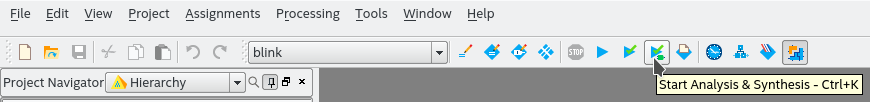
\includegraphics[scale=0.675]{39-start-analysis-synthesis-button}
\caption{Start Analysis and Synthesis Button on Intel Quartus Software Toolbar}
\label{fig:39-start-analysis-synthesis-button}
\end{figure}

\item The new top level module declares many more inputs and outputs than the First Qsys Design, so new pin constraints will need to be assigned to those pins.  The Terasic DE10-Nano user manual contains the diagrams and schematics where these pin assignments are derived from.  To make this process less error prone and faster we will copy the TCL commands below into a TCL script file that we name \textbf{hps\_pin\_assignments.tcl} that we create in the top level of the Intel Quartus software project directory:
\newline
\newline
%Extract PDF Attachment: \textattachfile[
%	color=0.0 0.678 0.937,
%	mimetype=text/plain,
%	description={TCL Source File: hps\_pin\_assignments.tcl}
%]{../hps_pin_assignments.tcl}{\textbf{hps\_pin\_assignments.tcl}}
Download the hps\_pin\_assignments.tcl file \href{\TheRawURL/MyFirstHPSSystem/writeup_MyFirstHPSSystem/hps_pin_assignments.tcl}{\underline{here}}.
\newline
If you wish to view the hps\_pin\_assignments.tcl file in the GitHub repo you can look \href{\TheBlobURL/MyFirstHPSSystem/writeup_MyFirstHPSSystem/hps_pin_assignments.tcl}{\underline{here}}.

\inputminted[
	bgcolor=MyMintedBGColor,
	linenos,
	fontsize=\footnotesize
]{tcl}{../hps_pin_assignments.tcl}

\newpage

\item With the \textbf{hps\_pin\_assignments.tcl} file created, we can now run it.  Begin by selecting the \textbf{TCL Scripts...} menu from the \textbf{Tools} menu as shown here:

\begin{figure}[H]
\centering
% screen shots report a density of 37.8 PixelsPerCentimeter when actual resolution
% is more like 56 PixelsPerCentimeter, so the scaling factor for 1:1 is 0.675
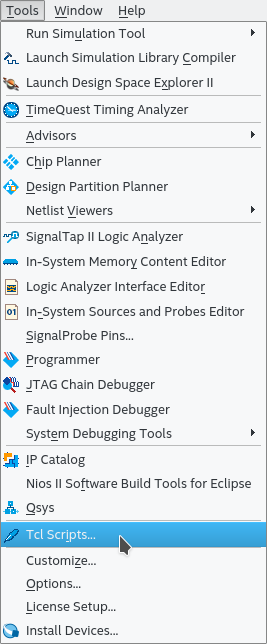
\includegraphics[scale=0.675]{36-quartus-tcl-scripts-menu}
\caption{TCL Scripts Menu}
\label{fig:36-quartus-tcl-scripts-menu}
\end{figure}

Then locate the \textbf{hps\_pin\_assignments.tcl} script in the dialog and select it and click the \textbf{Run} button.

\begin{figure}[H]
\centering
% screen shots report a density of 37.8 PixelsPerCentimeter when actual resolution
% is more like 56 PixelsPerCentimeter, so the scaling factor for 1:1 is 0.675
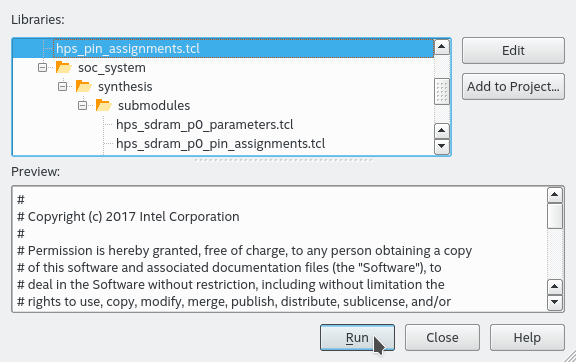
\includegraphics[scale=0.675]{37-run-hps-pin-assignments}
\caption{Run HPS Pin Assignments Script}
\label{fig:37-run-hps-pin-assignments}
\end{figure}

\newpage

\item Next we need to run the \textbf{hps\_sdram\_p0\_pin\_assignments.tcl} script that was generated by Qsys.  Begin by selecting the \textbf{TCL Scripts...} menu from the \textbf{Tools} menu as shown above, then locate the \textbf{hps\_sdram\_p0\_pin\_assignments.tcl} script in the dialog and select it and click the \textbf{Run} button.

\begin{figure}[H]
\centering
% screen shots report a density of 37.8 PixelsPerCentimeter when actual resolution
% is more like 56 PixelsPerCentimeter, so the scaling factor for 1:1 is 0.675
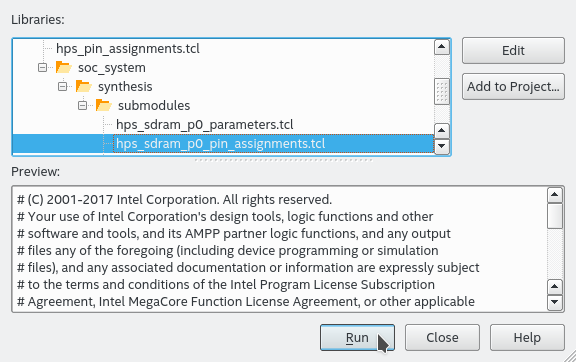
\includegraphics[scale=0.675]{38-run-hps-sdram-pin-assignments}
\caption{Run HPS SDRAM Pin Assignments Script}
\label{fig:38-run-hps-sdram-pin-assignments}
\end{figure}

\item Update the \textbf{blink.sdc} with the following code:
\newline
\newline
%Extract PDF Attachment: \textattachfile[
%	color=0.0 0.678 0.937,
%	mimetype=text/plain,
%	description={SDC Source File: blink.sdc}
%]{../../hdl_src/blink.sdc}{\textbf{blink.sdc}}
Download the blink.sdc file \href{\TheRawURL/MyFirstHPSSystem/hdl_src/blink.sdc}{\underline{here}}.
\newline
If you wish to view the blink.sdc file in the GitHub repo you can look \href{\TheBlobURL/MyFirstHPSSystem/hdl_src/blink.sdc}{\underline{here}}.

\inputminted[
	bgcolor=MyMintedBGColor,
	fontsize=\footnotesize,
	linenos
]{tcl}{../../hdl_src/blink.sdc}

\item Click the \textbf{Start Compilation} button in the top toolbar to compile the entire design.

\begin{figure}[H]
\centering
% screen shots report a density of 37.8 PixelsPerCentimeter when actual resolution
% is more like 56 PixelsPerCentimeter, so the scaling factor for 1:1 is 0.675
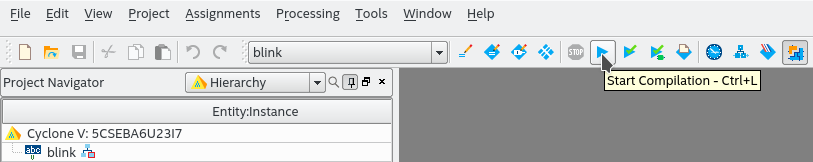
\includegraphics[scale=0.675]{14-start-compilation}
\caption{Start Compilation Button on Intel Quartus Software Toolbar}
\label{fig:14-start-compilation}
\end{figure}

\newpage

\item After your design has successfully compiled in the Intel Quartus software, you need to generate the Raw Binary File (RBF) that is used to program the FPGA from the HPS processor.  Begin by selecting the \textbf{File} menu and then select the \textbf{Convert Programming Files...} menu.

\begin{figure}[H]
\centering
% screen shots report a density of 37.8 PixelsPerCentimeter when actual resolution
% is more like 56 PixelsPerCentimeter, so the scaling factor for 1:1 is 0.675
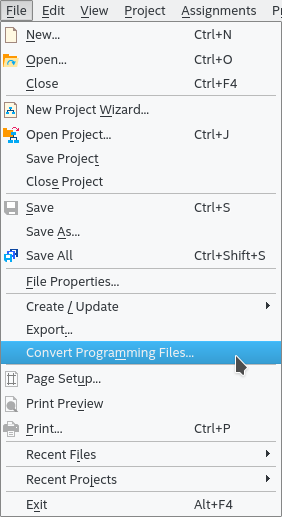
\includegraphics[scale=0.675]{40-cpf-menu}
\caption{Convert Programming Files Menu}
\label{fig:40-cpf-menu}
\end{figure}

\newpage

In the \textbf{Convert Programming Files} dialog perform the following actions:

\begin{enumerate}[
	label=\textbf{Step \arabic{enumi}\alph*.},
	leftmargin=*,
	align=left]

\item Change the \textbf{Programming file type} setting to \textbf{Raw Binary File(.rbf)}.

\item Change the \textbf{File name} setting to \textbf{output\_files/blink.rbf}.

\item Select the \textbf{SOF Data} entry in the \textbf{Input files to convert} table.

\item Click the \textbf{Add File...} button.

\item Browse to the \textbf{blink.sof} in the \textbf{output\_files} directory and select it.

\item Click the open button to close the file browser dialog and add that file to the list.

\item Click the \textbf{Generate} button to create the RBF file.

\item Close the \textbf{Convert Programming Files} dialog.

\end{enumerate}

\begin{figure}[H]
\centering
% screen shots report a density of 37.8 PixelsPerCentimeter when actual resolution
% is more like 56 PixelsPerCentimeter, so the scaling factor for 1:1 is 0.675
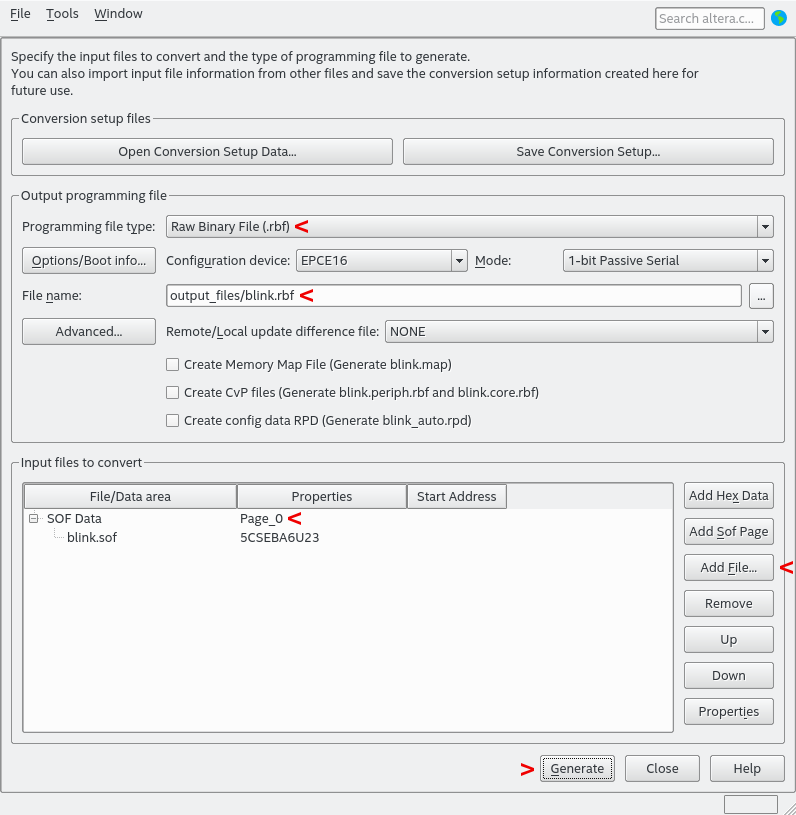
\includegraphics[scale=0.675]{41-convert-programming-files}
\caption{Convert Programming Files Menu}
\label{fig:41-convert-programming-files}
\end{figure}

\item Now let's perform one last activity in the Intel Quartus software to prepare for the next tutorial that will actually make use of this system on the Terasic DE10-Nano board.  Since we have defined a memory mapped embedded system in Qsys with a couple HPS masters connected to a number of slave peripherals, it will be necessary for us to know what the base addresses are of the slave peripherals so we can interact with them, performing read and write transactions to them.  That base address information is captured in Qsys, you can visualize that in Qsys a number of ways but that is not convenient for software developers or other users of this system to write code for it.  Each time you generate a Qsys system Qsys outputs a database file called \textbf{<your-\allowbreak system-\allowbreak name>.sopcinfo}.  The Intel Quartus software tools installation provides a utility that can be used to translate the SOPCINFO database information into a usable macro format that can be used for various purposes called \textbf{sopc-create-header-files}.  The default functionality of \textbf{sopc-\allowbreak create-\allowbreak header-\allowbreak files} is to create C style header macros from each masters perspective in the Qsys system.  We will perform this operation in the Intel Quartus software TCL Console which is located in the lower middle of the default Intel Quartus software GUI.  If you do not see the TCL Console pane, you can open it by selecting the \textbf{View} > \textbf{Utility Windows} > \textbf{TCL Console} menu.

\begin{figure}[H]
\centering
% screen shots report a density of 37.8 PixelsPerCentimeter when actual resolution
% is more like 56 PixelsPerCentimeter, so the scaling factor for 1:1 is 0.675
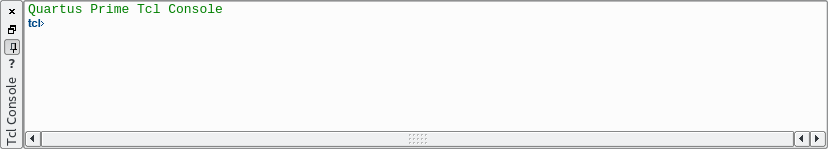
\includegraphics[scale=0.675]{15-tcl-console}
\caption{Intel Quartus Prime Software TCL Console}
\label{fig:15-tcl-console}
\end{figure}

We will first create a directory to output the header files into, then we will create the default header file output using \textbf{sopc-create-header-files} and finally we will extract the base address entries out of the HPS masters header file for the FPGA peripherals that they are connected to.  We will perform all of this with the following TCL commands:

\begin{minted}[
	fontsize=\footnotesize,
	bgcolor=MyMintedBGColor,
	escapeinside=++
]{text}

Quartus Prime Tcl Console

# make a directory called 'qsys_headers' to store the header files
tcl> file mkdir qsys_headers

# create a TCL variable SCHF_PATH to hold the path to the executable program
# sopc-create-header-files on your host PC using the environment variables
# provided by Quartus.
tcl> set SCHF_PATH [glob -join +\$+quartus(quartus_rootpath) sopc_builder bin sopc-create-header-files]

# create a TCL variable BAT_PATH to hold the path to the Nios II Command Shell
# batch file on Windows platforms.  The following code sequence will work on
# either Windows or Linux.  For linux this variable will just be set to NULL.
tcl> set BAT_PATH {}
tcl> if {+\$+tcl_platform(platform) == "windows"} {
   > set BAT_PATH [glob -join +\$+quartus(quartus_rootpath) .. nios2eds {Nios II Command Shell.bat}]
   > }

# execute sopc-create-header-files to generate the header files
tcl> eval exec -ignorestderr +\$+{BAT_PATH} +\$+{SCHF_PATH} soc_system.sopcinfo --output-dir qsys_headers

# read the header file for hps_0_arm_a9_0 into a TCL variable
tcl> set hps_0_arm_a9_0_header [read [open [glob -join qsys_headers hps_0_arm_a9_0.h] r]]

# output the C macro lines for the FPGA peripheral base addresses
tcl> foreach line [split +\$+{hps_0_arm_a9_0_header} "\n"] { \
   > if {[string match "*_BASE*" +\$+{line}]} { \
   > if {! [string match "*HPS_*" +\$+{line}]} {puts +\$+{line}}}}

\end{minted}

If you have put your Qsys system together properly and executed the above commands correctly, you should see the following output in the Intel Quartus software TCL console representing the base address definitions for the five Qsys peripherals in the FPGA fabric connected to the HPS H2F and LWH2F bridges.

\begin{minted}[
	bgcolor=MyMintedBGColor,
	escapeinside=++
]{c}

#define OCRAM_64K_BASE 0xc0000000
#define LED_PIO_BASE 0xff210000
#define BUTTON_PIO_BASE 0xff210010
#define SWITCH_PIO_BASE 0xff210020
#define SYSTEM_ID_BASE 0xff210030

\end{minted}

\end{enumerate}

\newpage

That's it! You have designed and compiled your first HPS system.  Continue on to the \textquote{Interacting with FPGA Designs Using U-Boot} tutorial where we demonstrate how to use U-Boot to program the FPGA and interact with this design.  Or you can continue on to the \textquote{Interacting with FPGA Designs Using Linux} tutorial where we demonstrate how to interact with this design from Linux.

\end{flushleft}

\end{document}

